\section{Implementazioni}
La memoria secondaria permette di mantenere una grande quantità di dati in modo permanente.
I \textbf{dischi magnetici} e i \textbf{dischi a stato solido} sono i due principali mezzi per la memorizzazione di massa.

\spacer
L'unità disco è connessa al calcolatore mediante un bus di I/O, il quale può essere di diversi tipi:
\begin{sitemize}
    \item \textbf{ATA} (Advanced Technology Attachment)
    \item \textbf{SATA} (Serial ATA)
    \item \textbf{USB}
    \item \textbf{Thunderbolt}
\end{sitemize}
\spacer
Sia dal lato del calcolatore che da quello del disco sono inseriti dei controllori per gestire il flusso di dati ed il disco.

Quando viene richiesta un'operazione I/O al disco i dati vengono prima copiati nella cache del disco e poi vegnono inviati alla RAM del sistema.

\subsection{HDD}
Un Hard Disk è composto da molti dischi paralleli impilati (piatti), su ogni piatto sono presenti numerosi anelli concentrici (traccie), ogni traccia viene divisa in settori.

Diremo cilindro l'insieme di tutte le traccie poste alla stessa distanza dal centro, mentre un blocco è l'insieme di tutti i settori posti nella stessa posizione in tutti i piatti.

\begin{figure}[H]
    \centering
    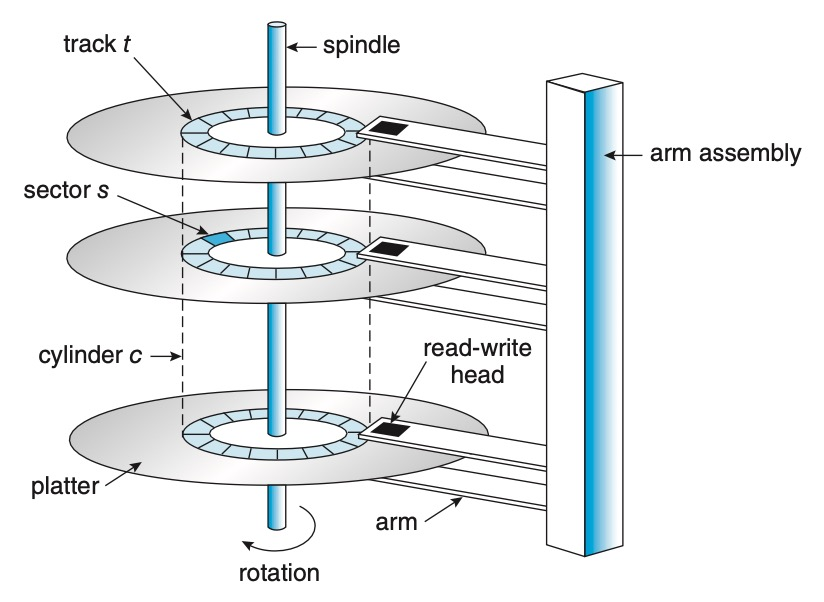
\includegraphics[width=0.5\linewidth]{assets/hdd.jpg}
\end{figure}

Ogni piatto ha una testina che ha il compito di lettura/scrittura sul disco. La maggior parte della latenza dei dischi rigidi è dovuta allo spostamento di questo elemento.

Negli anni quasi tutte le proprietà del disco sono state migliorare sostanzialmente, con l'eccezione del tempo di accesso, dettato da limitazioni fisiche.

\begin{figure}[H]
    \centering
    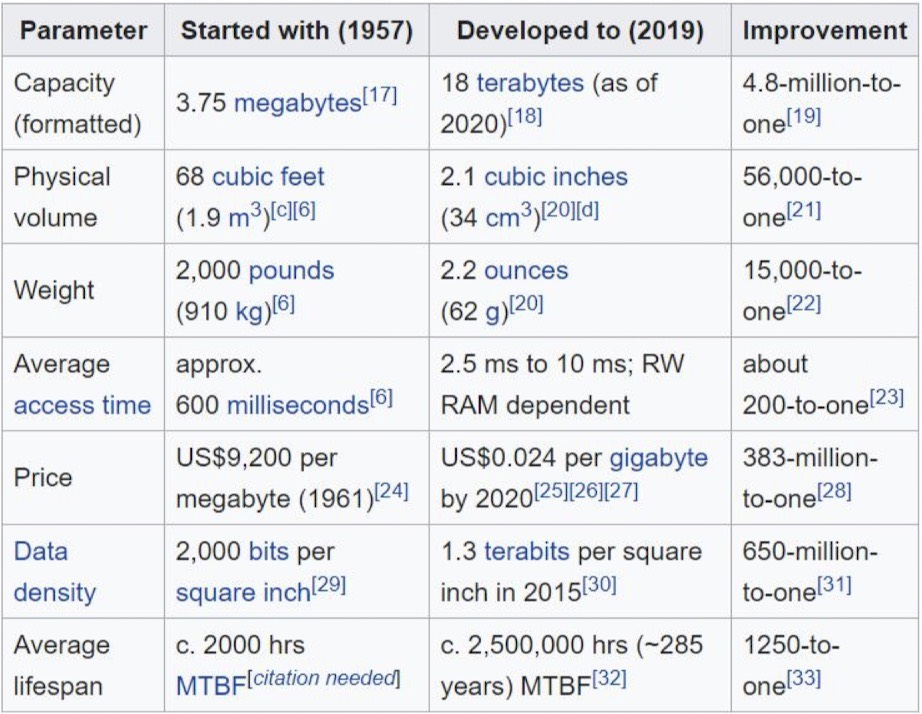
\includegraphics[width=0.5\linewidth]{assets/hdd-improvement.jpg}
\end{figure}

\subsubsection{Implementazioni}
\begin{sitemize}
    \item \textbf{CAV} \textit{Constant Angular Velocity}, la velocità di rotazione resta costante per ogni traccia, così come la quantità di dati per ogni traccia. Questo significa che traccie più interne devono avere maggiore densità.
    \item \textbf{CLV} \textit{Constant Linear Velocity} La densità rimane costante su tutto il disco, questo significa che la velocità angolare deve aumentare quando ci si sposta da traccie esterne a quelle interne.
\end{sitemize}

\begin{figure}[H]
    \centering
    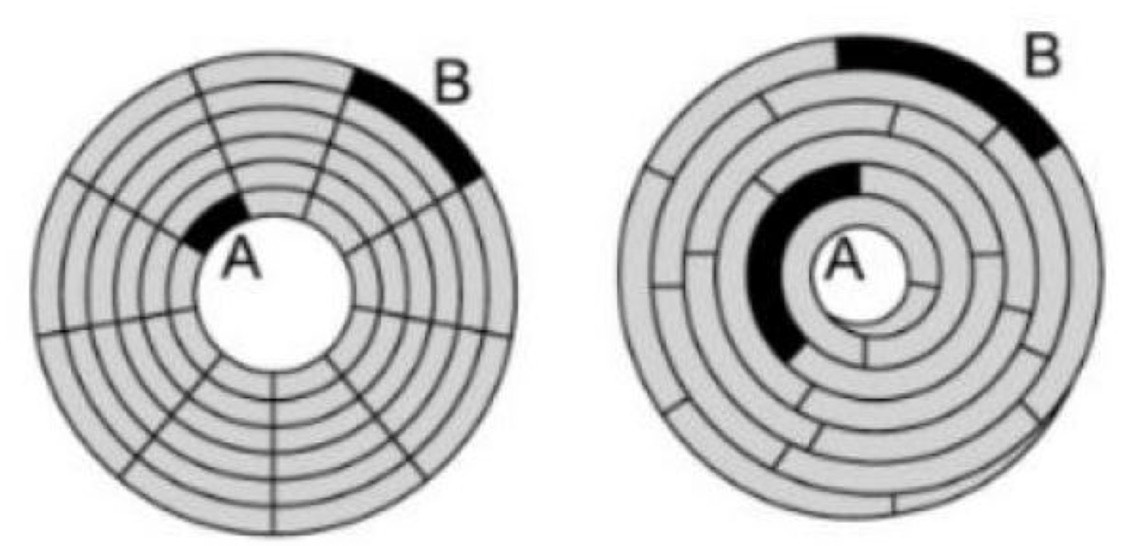
\includegraphics[width=0.5\linewidth]{assets/cav-clv.jpg}
    \caption{CAV a sinistra, CLV a destra}
\end{figure}

\begin{note}
    Un esempio visivo di encoding dei dati su un disco si può trovare nel paracadute usato dalla sonda \textit{Perseverance} durante il suo atterraggio su Marte nel 2021.

    Su di esso è presente un codice binario che si può leggere come un disco magnetico e riporta il motto "dare mighty things".

    \begin{figure}[H]
        \centering
        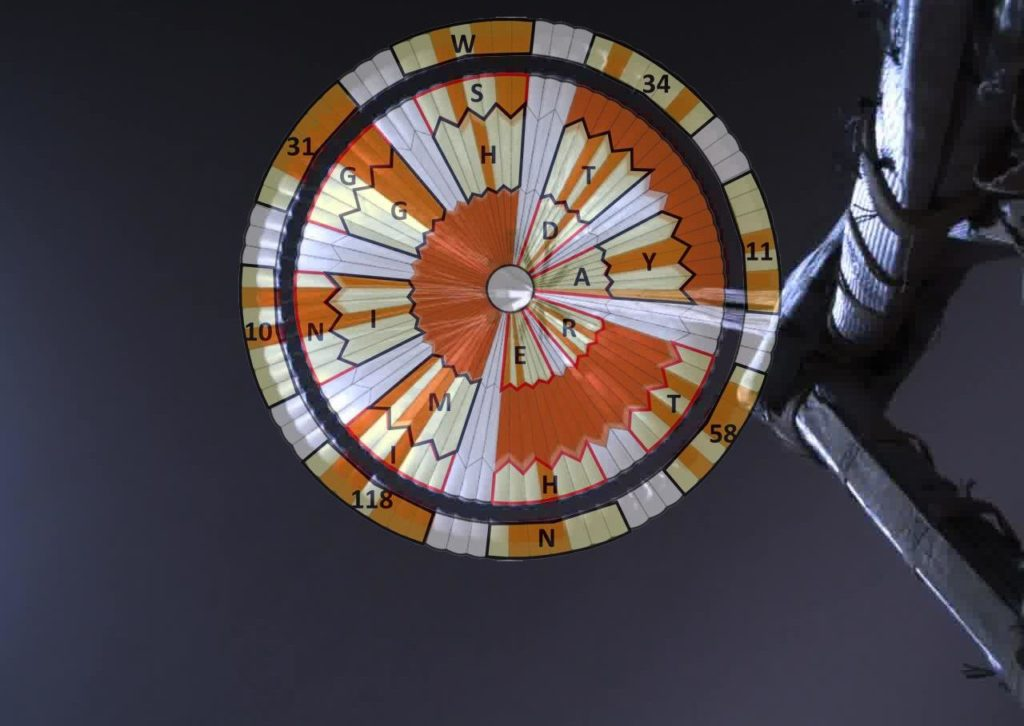
\includegraphics[width=0.6\linewidth]{assets/perseverance.jpg}
    \end{figure}
\end{note}

\subsubsection{Scheduling}
Le prestazioni degli algoritmi di scheduling vengono misurate su una coda di richieste per i cilindri 98, 183, 37, 122, 14, 124, 65, 67, con la testina inizialmente impostata sul cilindro 53.

\begin{figure}[H]
    \centering
    \begin{minipage}{0.5\textwidth}
        \subsubsection*{First Come First Serve}
        Un algoritmo spesso inefficiente in quanto può risultare in grandi oscillazioni, in questo caso muove la testina di 640 cilindri.
    \end{minipage}
    \hfill
    \begin{minipage}{0.4\textwidth}
        \begin{figure}[H]
            \centering
            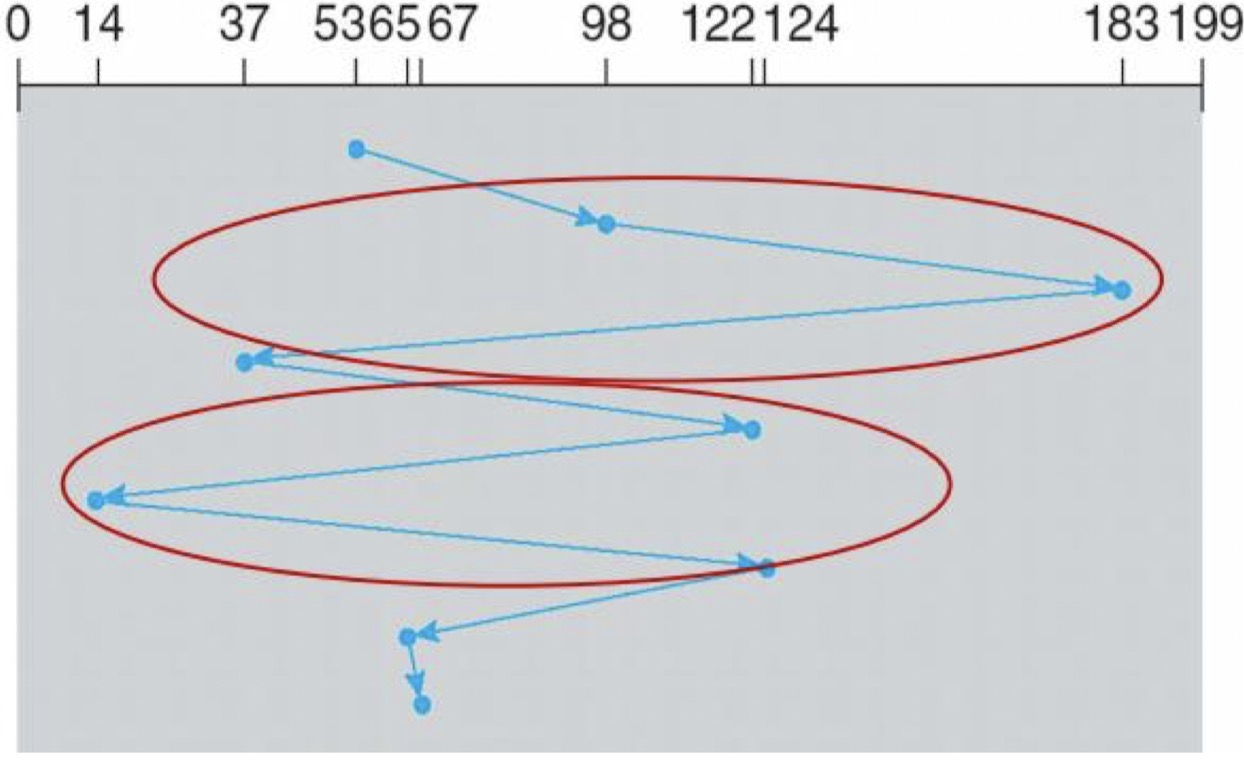
\includegraphics[width=1\linewidth]{assets/fcfs.jpg}
        \end{figure}
    \end{minipage}
\end{figure}

\begin{figure}[H]
    \centering
    \begin{minipage}{0.5\textwidth}
        \subsubsection*{Shortest Seek Time First}
        Si muove sempre verso l'elemento più vicino, questo può causare l'attesa indefinita di alcune richieste e non è ancora ottimale. In questo caso muove la testina di 236 cilindri.
    \end{minipage}
    \hfill
    \begin{minipage}{0.4\textwidth}
        \begin{figure}[H]
            \centering
            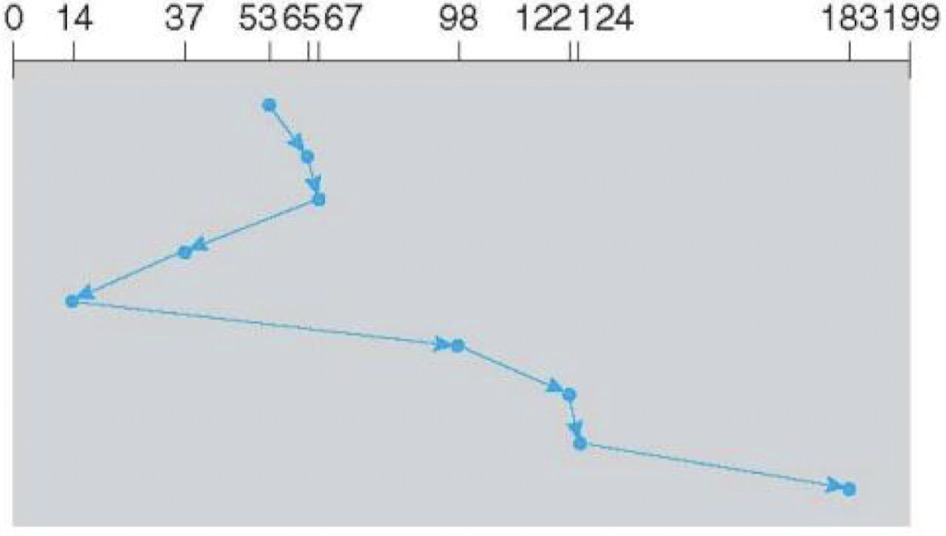
\includegraphics[width=1\linewidth]{assets/sstf.jpg}
        \end{figure}
    \end{minipage}
\end{figure}

\begin{figure}[H]
    \centering
    \begin{minipage}{0.5\textwidth}
        \subsubsection*{Scan}
        Il braccio della testina si muove da un estremo all'altro, servendo le richieste che incontra.

        Una variante di questo algoritmo, detta look, ferma lo scanning prima della fine, all'ultimo cilindro richiesto. Questo richiede dell'overhead per controllare la coda, ma riduce il numero di spostamenti sprecati.
    \end{minipage}
    \hfill
    \begin{minipage}{0.4\textwidth}
        \begin{figure}[H]
            \centering
            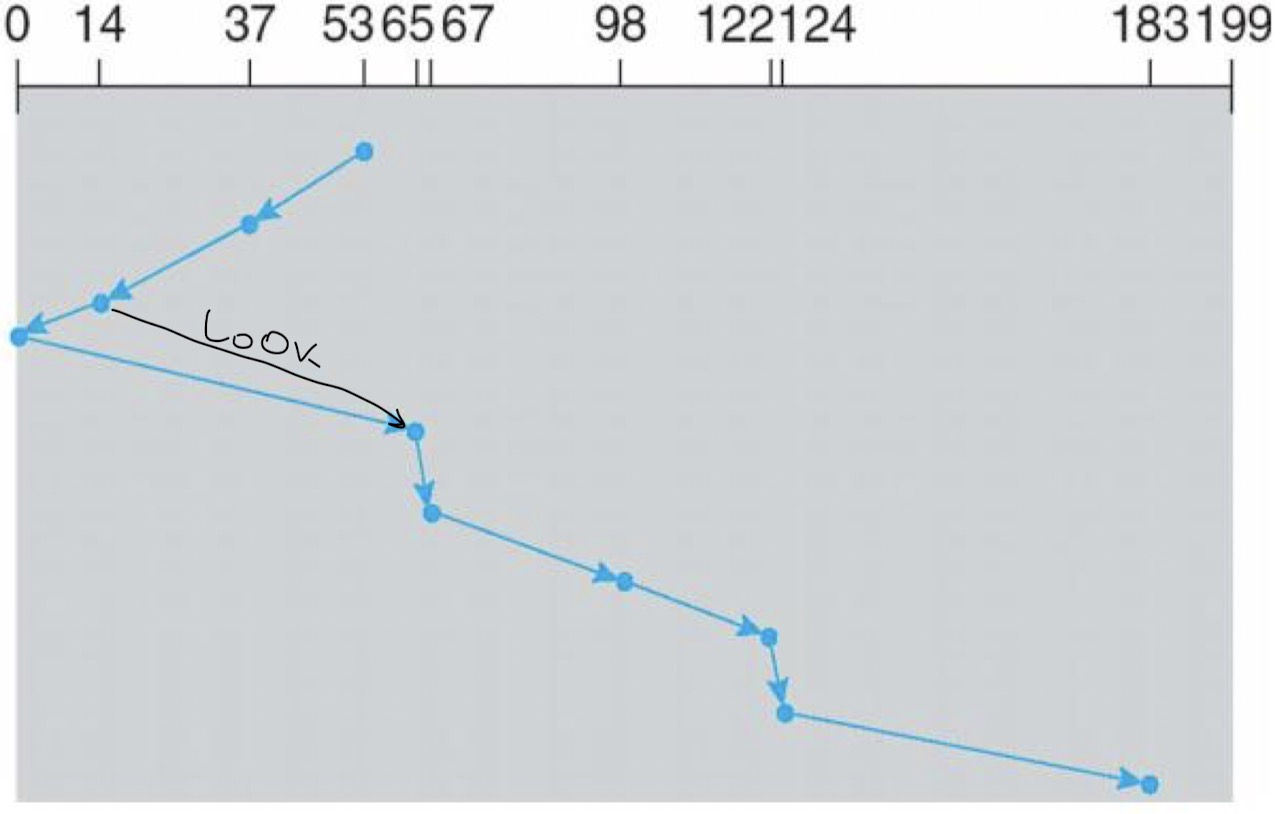
\includegraphics[width=1\linewidth]{assets/scan.jpg}
        \end{figure}
    \end{minipage}
\end{figure}

\begin{figure}[H]
    \centering
    \begin{minipage}{0.5\textwidth}
        \subsubsection*{C-Scan}
        Simile a Scan, ma la testina compie richieste solo in una direzione, per poi ritornare velocemente all'altro estremo. Questo fornisce un tempo di attesa più uniforme.
    \end{minipage}
    \hfill
    \begin{minipage}{0.4\textwidth}
        \begin{figure}[H]
            \centering
            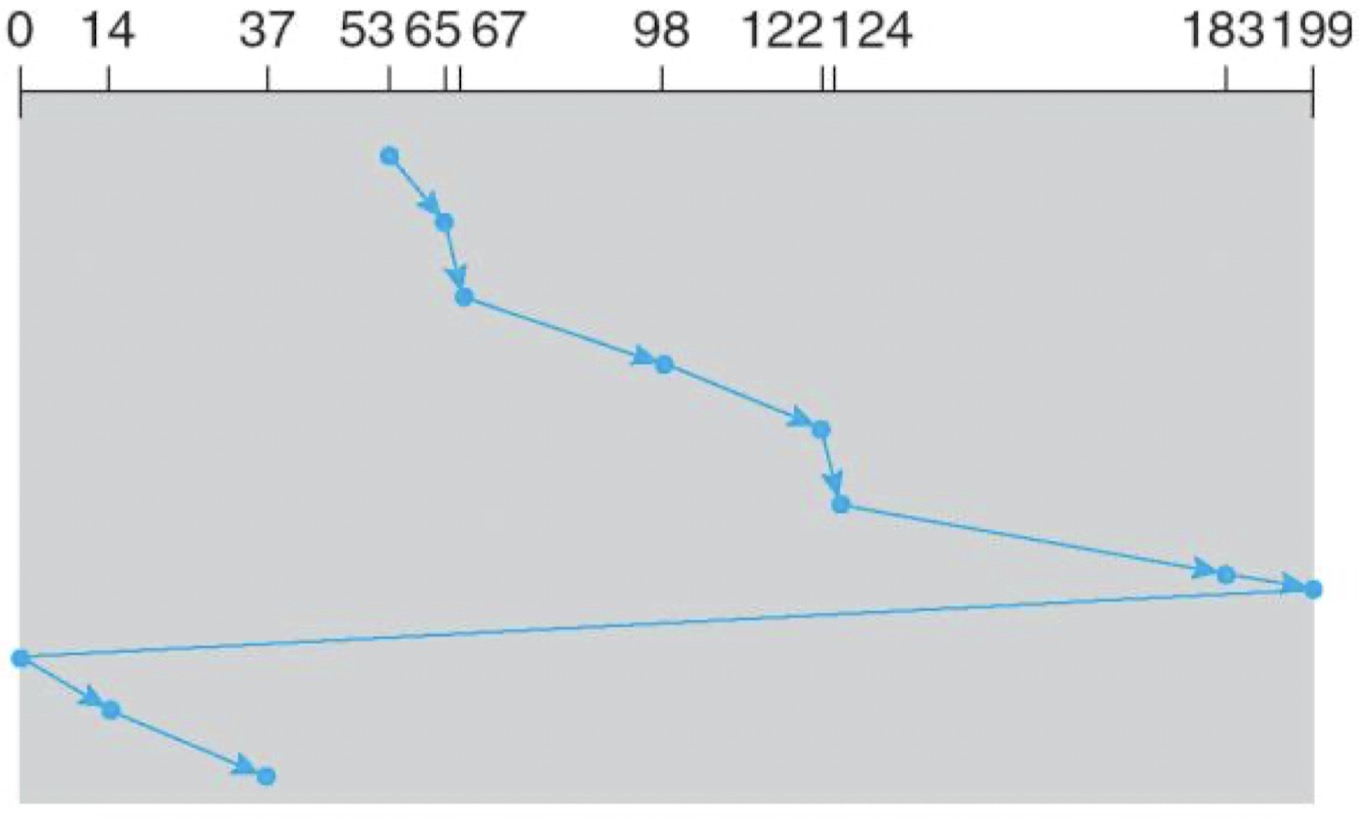
\includegraphics[width=1\linewidth]{assets/c-scan.jpg}
        \end{figure}
    \end{minipage}
\end{figure}

\begin{figure}[H]
    \centering
    \begin{minipage}{0.5\textwidth}
        \subsubsection*{C-Look}
        Una versione ottimizzata di c-scan che si ferma all'ultima richiesta senza arrivare alla fine dei cilindri.
    \end{minipage}
    \hfill
    \begin{minipage}{0.4\textwidth}
        \begin{figure}[H]
            \centering
            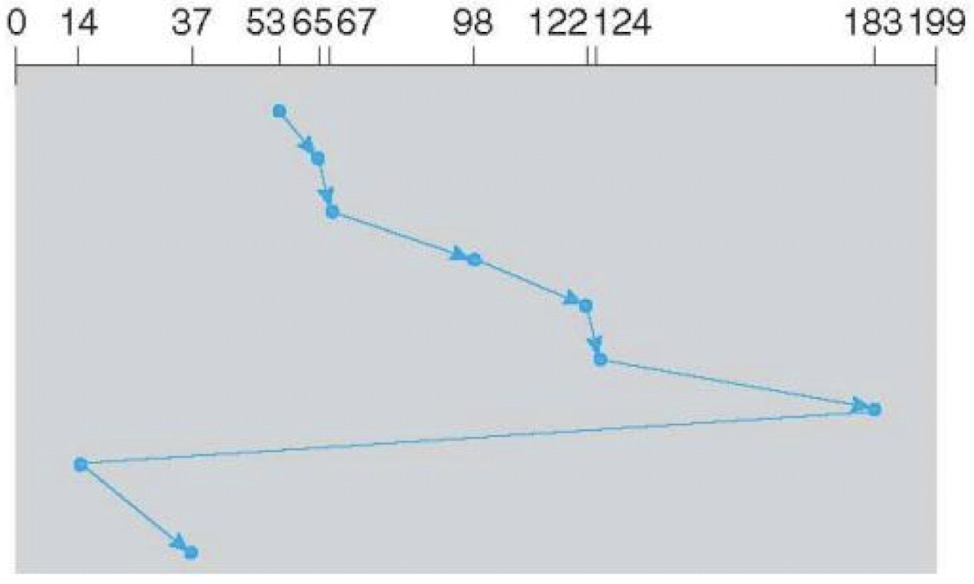
\includegraphics[width=1\linewidth]{assets/c-look.jpg}
        \end{figure}
    \end{minipage}
\end{figure}

Nei sistemi operativi moderni spesso non vale la pena di ottimizzare in modo particolare gli algoritmi di scheduling, viene quindi spesso utilizzato Shortest Seek Time First, con qualche accorgimento per evitare lo starving.

\subsection{SSD}
Sono delle memorie a stato solido, costituite a da transistor MOSFET i quali sono in grado di mantenere una determinata carica elettrica per un lungo tempo.
\spacer
Nei nuovi dischi è possibile memorizzare nei transistor più livelli di tensione (oltre al solito 0 o 5V). In questo modo si aumenta notevolmente la densità, ma aumenta anche la complessità.

\spacer
I dischi a stato solido hanno tempo di accesso costante per ogni cella, quindi la frammentazione del disco non è più problematica.

\spacer
Al contrario ai dischi magnetici le memorie a stato solido non possono essere sovrascritte, è necessario riportare tutti i bit a 0 e poi scrivere nuovi dati.
A questo si aggiunge il fatto che la scrittura dei dati è la principale causa di fallimento del disco, tuttavia grazie alle nuove tecnologie si è riusciti a limitare questo problema.

\begin{figure}[H]
    \centering
    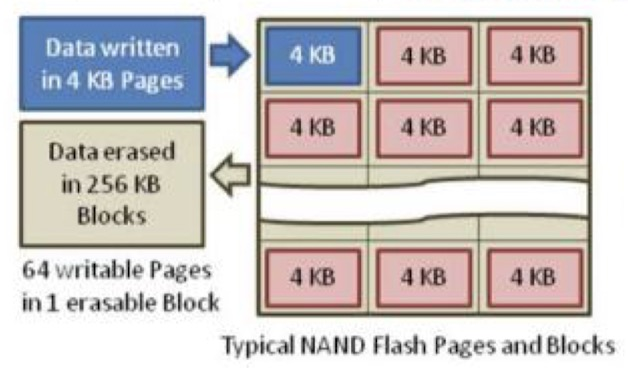
\includegraphics[width=0.5\linewidth]{assets/SSD.jpg}
    \caption{Disco rigido con pagine da 4KB e blocchi di eliminazione da 256KB}
\end{figure}

Per il fatto che i blocchi di eliminazione sono più grandi delle pagine può essere necessario copiare alcuni elementi in un'altro blocco prima di effettuare l'eliminazione.

\subsection{Tape}
I nastri magnetici sono ancora utilizzati per alcune specifiche applicazioni, in particolare di backup.
Essi infatti, se tenuti correttamente, possono durare per ~100 anni e sono estremamente capienti (i più nuovi fino a 580 Tb).

Essi sono prettamente sequenziali, quindi il tempo di accesso è spesso molto elevato.

\subsection{DNA}
Sembra che il futuro della memorizzazione dei dati si trovi nel DNA, il quale può essere utilizzato per archiviare enormi quantità di dati per un periodo di tempo estremamente lungo (215 petabyte in 1 grammo per migliaia di anni).

\spacer
Per ora è una tecnica che ha ancora costi proibitivi, per scrivere 2 megabyte sono necessari 7000 dollari e altri 2000 per leggerli.
